\documentclass{bmvc2k}

\usepackage{graphicx}
\graphicspath{ {./Figs/} }
\usepackage{amsmath}
\usepackage{amsfonts}

%% Enter your paper number here for the review copy
% \bmvcreviewcopy{??}

% \usepackage[brazilian]{babel}
\usepackage[utf8]{inputenc}

\title{Project 2 - Deep fake detection}

% Enter the paper's authors in order
% \addauthor{Name}{email/homepage}{INSTITUTION_CODE}
\addauthor{Christian Miranda}{christianmoryah@gmail.com}{1}

% Enter the institutions
% \addinstitution{Name\\Address}
\addinstitution{
  Departamento de Ci\^encia da Computa\c{c}\~ao\\
  Universidade de Bras\'{\i}lia\\
  Campus Darcy Ribeiro, Asa Norte\\
  Bras\'{\i}lia-DF, CEP 70910-900, Brazil 
}

\runninghead{Student, de Campos}{Computer Vision Assignment -- \today}

% Any macro definitions you would like to include
% These are not defined in the style file, because they don't begin
% with \bmva, so they might conflict with the user's own macros.
% The \bmvaOneDot macro adds a full stop unless there is one in the
% text already.
\def\eg{\emph{e.g}\bmvaOneDot}
\def\Eg{\emph{E.g}\bmvaOneDot}
\def\etal{\emph{et al}\bmvaOneDot}

%-------------------------------------------------------------------------
% Document starts here
\begin{document}

\maketitle

\begin{abstract}
Deep fakes have been gaining more popularity every year. Thanks to new advanced machine learning techniques, the quality of deep fakes has increased so much that many have become difficult to detect fake faces even for humans.

Due to this growth in popularity, research in the area has increased considerably, resulting recently in deep fake detection challenges on Kaggle, with thousands of participants.

Considering the race between deep fakes generators and discriminators, this work aims to 1: collect relevant deep fake image data sets for experimentation, and 2: compare different techniques for detecting deep fake generated faces on the collected data.

% {\bf All authors are encouraged to read this document}, even if you have
% written many papers before.  As well as a description of the format, the
% document contains many instructions relating to formatting problems and
% errors that are common even in the work of authors who {\em have}
% written many papers before.
\end{abstract}

%-------------------------------------------------------------------------
\section{Introduction}
\label{sec:intro}

Deep fake is a synthetic media generated by deep learning models. The goal is to replace a person's image or voice with another person's data.

For the production of quality deep fakes, current state of the art techniques implement a neural network architecture called Generative Adversarial Networks (GAN) \cite{goodfellow_generative_2014}. In this technique, we have 2 neural networks working in parallel: The Generator and the Discriminator.

The Generator is the neural network that learns to generate the fake media, and the Discriminator is the neural network that learns to detect them.

The training is carried out in parallel: the generator receives random noise as input and tries to create realistic images. Its learning is linked to the learning of the Discriminator. When the generated image is detected, it performs the adjustment of its parameters through gradient descent. 

The Discriminator, on the other hand, needs to learn to detect the fake photos of the real ones, for that, he receives input from 2 sources: photos from the generator and real photos. Its parameters are adjusted according to the failure to detect forgeries, or when it believes that a real photo is fake. Figure 1 shows the general architecture of GAN networks.

\begin{figure}[!h]
\centering
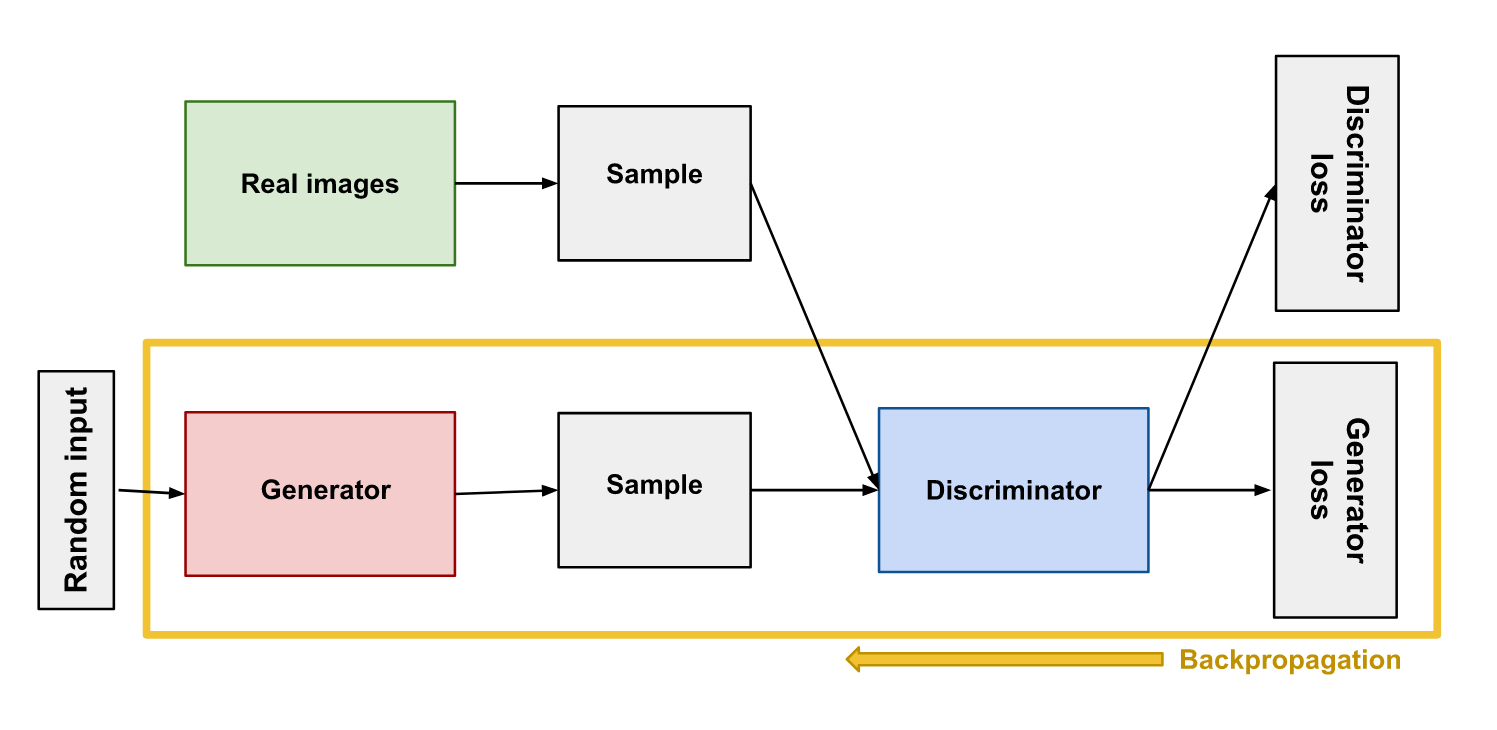
\includegraphics[width=7.5cm, height=3.8cm]{GAN.png}
    \caption{Architecture of a GAN network pair}
\end{figure}

\section{Related Work}

Image forgery detection methods embrace a wide range of approaches that can be divided in two categories:
1. extrinsic features and 2. intrinsic features. The first one will embed external unique signals in the original images, like digital watermarks, but its complex to implement, since all pictures would now have to embed this extra information. Intrinsic features strategy tries to find the invariant features directly from the images, and it is the selected method for this work.

Considering the intrinsic feature strategy, there are several methods, that can be classified according to the features that they target. The simplest method is: Using deep convolutional neural network (CNN) based detection models to capture the image and face features but in an inexplicit way (using the deep CNN parameter weights). 

Other notable approaches are: 1. Spectral decomposition of the images using Fourier transform \cite{durall2019unmasking} which will be used in this work, 2. Illumination modeling \cite{journals/tifs/CarvalhoRAPR13}, that targets illumination inconsistencies on generated images (but this is a method from 2012, before the "GAN spring", and not specific for fake face detection), 3. Eye blinking detection \cite{journals/corr/abs-1806-02877}, which takes advantage of the fact that deep fake faces rarely blink on videos, since the input training images / videos have very few frames of people blinking.


\section{Methodology}
\label{sec:depth}
In this work, we will do the following steps:

\begin{itemize}
  \item Gather data from different sources for the analysis;
  \item Select one or more appropriate models for testing on the data set, the models may be pretrained or not.
  \item Test the models on the data and compare the results
\end{itemize}

\subsection{Gathering Deep Fake data}

Kaggle hosted a major deep fake detection challenge in 2020 and created a new data set for it \cite{dolhansky2019deepfake}. This data was chosen because of its popularity, but only a subset was used:  the 'Preview data set', containing 400 labeled videos. The challenge was about detecting deep fakes in video, so the face images had to be extracted from the original data set.

For this we used Paul Viola and Michael J. Jones "Robust real-time face detection" algorithm implemented in OpenCV \cite{violajones04}. The labeled train part of the data set (test videos could not be used as the were not labeled) generated a total of 1121 images, 918 fake and 203 real, a rather unbalanced data set but still usable.

\begin{figure}[!h]
\centering
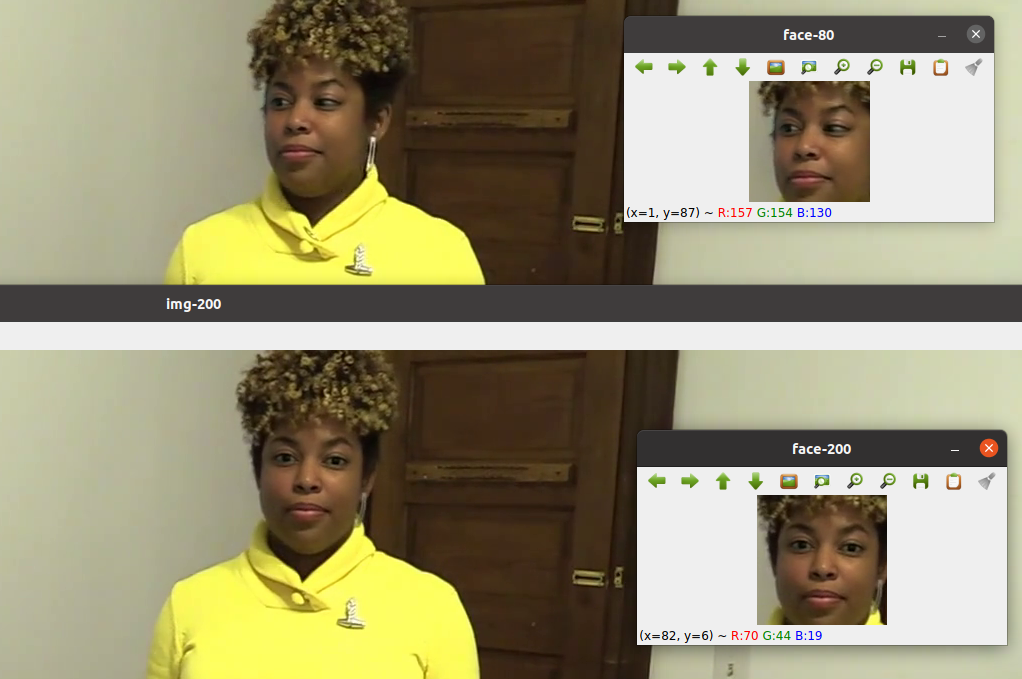
\includegraphics[width=7.0cm, height=4.3cm]{face-extraction.png}
    \caption{Faces being extracted from random video frames}
\end{figure}

Due to the excess artifacts generated on the face in certain frames by the deep fake algorithm, the Viola-Jones cascade classifier wasn't able to detect the face, so 78 frames were lost in this process.

\subsection{Choosing Deep Fake detection models}

As a result of bibliographic research, the following methods were selected for testing. Both methods were chosen by their simplicity and size. So they don't need the use of a GAN discriminator, or even a big CNN classifier:

\begin{itemize}
  \item "MesoNet: a Compact Facial Video Forgery Detection Network" \cite{journals/corr/abs-1809-00888};
  \item "Unmasking DeepFakes with simple Features" \cite{durall2019unmasking}.
\end{itemize}


The MesoNet pretrained detection model comes with a larger data set than the one generated in the previous section. Since this dataset was used in training and validation of the MesoNet Model, we decided not to use it in this work, considering that the model was tuned to better perform on its test data.

In \cite{journals/corr/abs-1809-00888}, the authors explain that a small CNN architecture can extract the features from images generated by different GAN architectures. These features are later fed to a dense classification network, where it is possible to obtain good classification results. The model architecture is available in Figure 3.

\begin{figure}[!h]
\centering
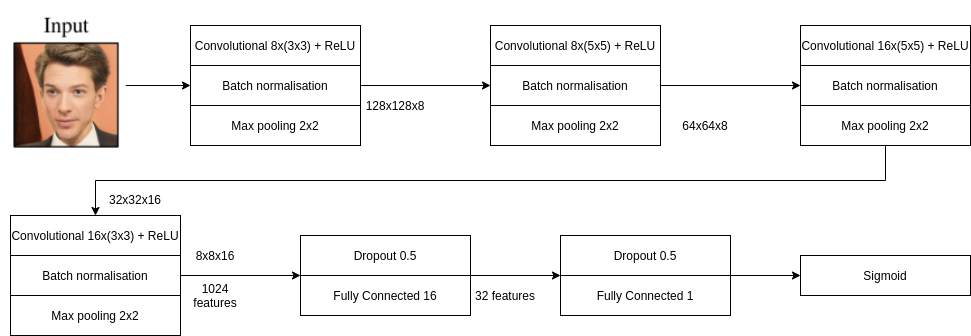
\includegraphics[width=7.5cm, height=3.0cm]{mesonet.png}
    \caption{Meso-4 network architecture}
\end{figure}


The training computation is defined by regular gradient descent, where the loss L can be computed by the Cross entropy formula:

\begin{equation}\label{eq:2}
 L = - \frac{1}{m} \sum_{i=1}^{m} y_i \cdot \log{\hat{y}_i}
\end{equation}

The y letter is the actual label, and ŷ is the classifier’s output. The cross entropy loss is the negative of the first, multiplied by the logarithm of the second. Also, m is the number of examples, so the total loss is the average loss over all the examples.

\hspace{1.5cm}

The second method, in turn, uses signal processing techniques from Frequency Domain Analysis for feature extraction, instead of relying on a CNN. 

The input face image is processed using a Discrete fourier transform, that decomposes the signal into sinusoidal components of various frequencies. It then passes trought an Azimuthal Average processing to compute a robust 1D representation of the DFT power spectrum, after that, 1D vector can be processed by any machine learning classifier (we will be using SVM and Logistic Regression, the same used in the original paper). Figure 4 shows the steps of the process.


\begin{figure}[!h]
\centering
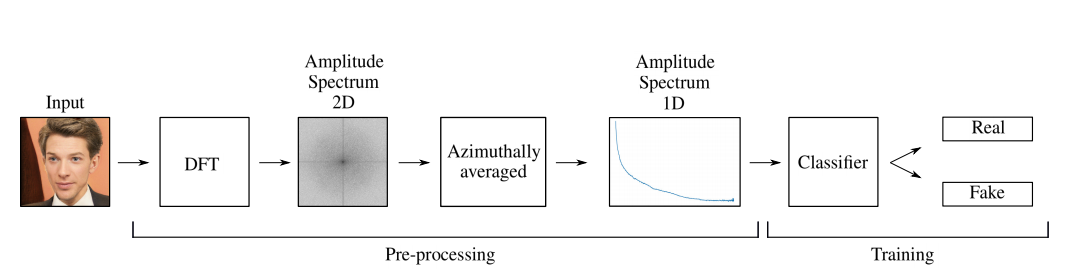
\includegraphics[width=8.6cm, height=3.0cm]{fft-pipeline.png}
    \caption{Discrete Fourier Transform pipeline}
\end{figure}


For each input picture of size M × N, the DFT can be computed as:

\begin{equation}\label{eq:1}
  X_{k,l} = \sum_{n=0}^{N - 1} \sum_{0}^{M- 1} X_{n,m} \cdot e^{\frac{-i2\pi}{ N} kn} \cdot e^{\frac{-i2\pi}{ M} lm}
\end{equation}

\subsection{Testing models on the data set}

The MesoNet Model is already pretrained, but we will further train it in the train part of the data set for another 10 epochs. We define the models architecture and load the pretrained weights (weights file size = 156KB) available in the original project, then perform the train stage.

It is noticeable that the model accuracy performance was already poor during training, the best accuracy at the end of epoch 10 was 0.66. Figure 5 shows model performance through epochs.

\begin{figure}[!h]
\centering
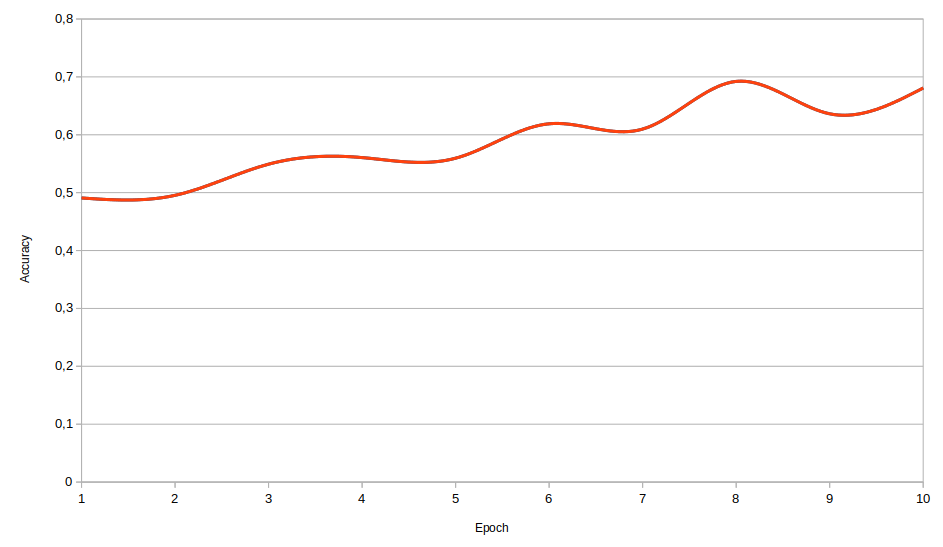
\includegraphics[width=8.6cm, height=3.0cm]{Figs/train-performance-mesonet.png}
    \caption{MesoNet performance - epochs 1 to 10}
\end{figure}

\hspace{1.5cm}

For the Discrete Fourier Transform method, we load the face images and process them through the pipeline. First we use the numpy DFT implementation to get the amplitude spectrum, and then apply Azimuthal Average to get the 1D Vectors representing the face features. The processed data is then saved to disk in pickle format for reusing. Total disk usage for all images in jpg format: 10MB. Total disk usage after feature extraction: 2.7MB.

After feature extraction, we split the data into train and validation sets and start training the models. Support Vector Machines and Logistic Regression are used for interpreting the extracted features.

\section{Results}

MesoNET model performed worse than expected, even after being trained on a piece of the current data set, test accuracy peaked at 53\%, almost the same as a random guess by the flip of a coin. The table below shows sklearn's classification report, and Figure 6 shows the models confusion matrix. As can be observed in the confusion matrix, the model is overfitted to believe that a large number of real photos are fake. Several tuning were made to obtain this performance, including increasing the epoch number and setting custom class weights, considering the imbalance of the data set.

\begin{center}
\begin{tabular}{ c c c c c }
  & precision & recall & f1-score & support \\
 fake & 0.80 & 0.58 & 0.67 & 183 \\ 
 real &  0.14 & 0.33 & 0.20 & 40 \\
 accuracy &  &  & 0.53 & 223
\end{tabular}
\end{center}


\begin{figure}[!h]
\centering
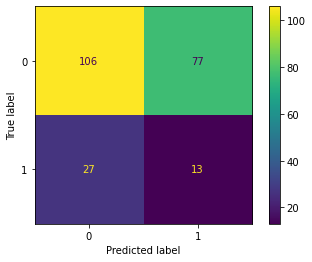
\includegraphics[width=4cm, height=4cm]{Figs/mesoNet-confusion-matrix.png}
    \caption{MesoNet confusion matrix}
\end{figure}

The second technique, on the other hand, performed much better. Even though this pipeline is really designed to work with high resolution images, it worked really well for this poor resolution data set. Logistic Regression model obtained 82\% accuracy and Support Vector Machines got 96\%. LR classification report is available in the table below. 

\begin{center}
\begin{tabular}{ c c c c c }
  & precision & recall & f1-score & support \\
 fake & 0.84 & 0.98 & 0.90 & 189 \\ 
 real &  0.00 & 0.00 & 0.00 & 36 \\
 accuracy &  &  & 0.82 & 225
\end{tabular}
\end{center}


\vspace{0.6cm} Table above shows that even though LR model got a good accuracy, it totally failed to guess the real faces, thinking that all of them were fake faces. SVM classification report:

\begin{center}
\begin{tabular}{ c c c c c }
  & precision & recall & f1-score & support \\
 fake & 0.97 & 0.97 & 0.97 & 189 \\ 
 real &  0.86 & 0.86 & 0.86 & 36 \\
 accuracy &  &  & 0.96 & 225
\end{tabular}
\end{center}

Both model confusion matrices can be checked in Figures 7 and 8 below.

\begin{figure}[!h]
  \centering
  \begin{minipage}[b]{0.4\textwidth}
    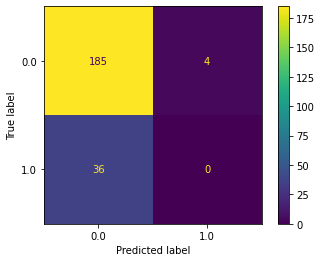
\includegraphics[width=4.3cm, height=4cm]{Figs/lr-confusion-matrix.png}
    \caption{LR confusion matrix}
  \end{minipage}
  \hfill
  \begin{minipage}[b]{0.4\textwidth}
    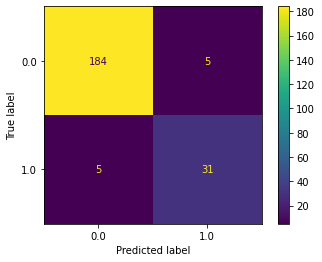
\includegraphics[width=4.3cm, height=4cm]{Figs/svm-confusion-matrix.png}
    \caption{SVM confusion matrix}
  \end{minipage}
\end{figure}

Finally, figure 9 shows some examples of faces being correctly classified as fakes.

\begin{figure}[!h]
\centering
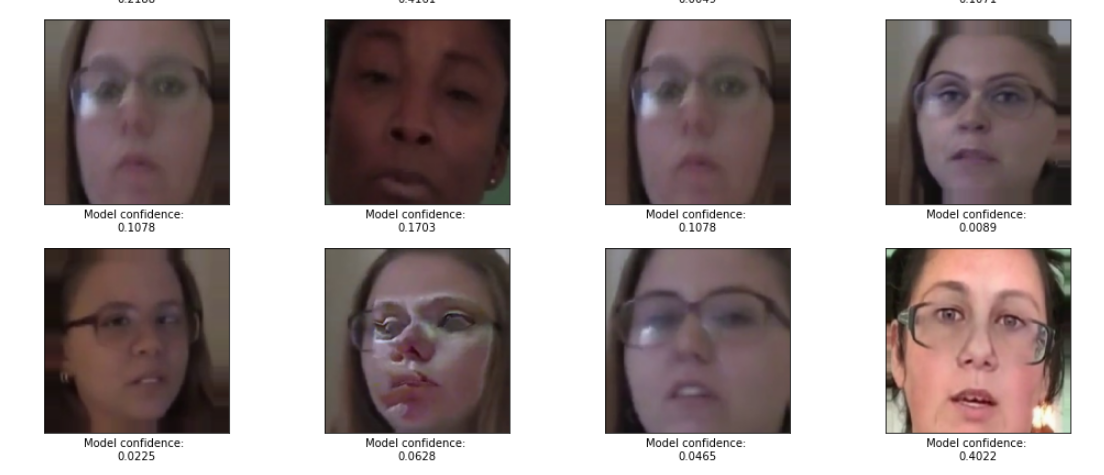
\includegraphics[width=9cm, height=4cm]{Figs/results.png}
    \caption{Deep fake faces classified as fake}
\end{figure}

\section{discussion and conclusions}

Contrary to our first hypothesis, MesoNET wasn't able to correctly generalize and predict real faces from fake ones. The model was later trained until 50 epochs to check if its performance could be better but without success, early stopping at 10 epochs still gave better results.

The composition DFT feature extraction, however, generated impressing results with the SVM model. accuracy values can be compared in the table below:

\begin{center}
\begin{tabular}{ c c }
 Model & Accuracy\\
 MesoNet & 0.53 \\ 
 DFT + LR & 0.82 \\
 DFT + SVM & 0.96
\end{tabular}
\end{center}

Even tough the selected models only work with images, it is possible to embed them in a video analysis and use them 'frame by frame'. In future works it is possible to join the data of the features extracted by each frame in a temporal sequence and use recurrent models (such as LSTM) or even Attention to also process the relationship between the frames, making the model even more stable.


\bibliography{refs}
\end{document}
